\begin{figure}[h!]
    \centering
    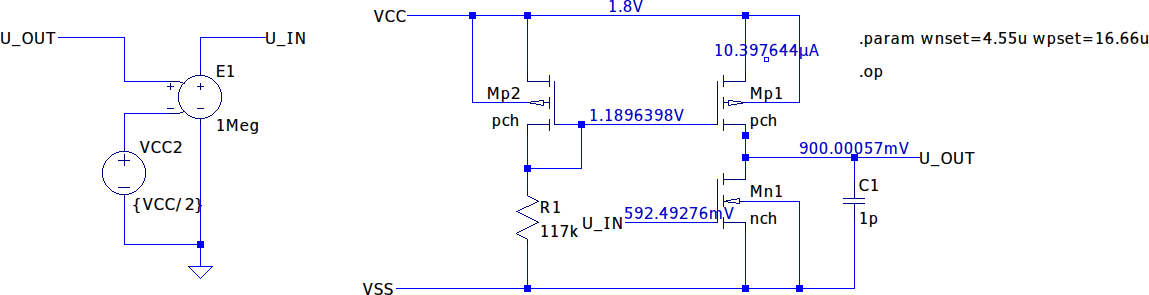
\includegraphics[scale=0.5]{4-2-1.png}
    \caption{Aktivní zátěž -- zapojení pro OP analýzu.}
    \label{fig:spice0-png}
  \end{figure}
  \begin{figure}[h!]
      \centering
      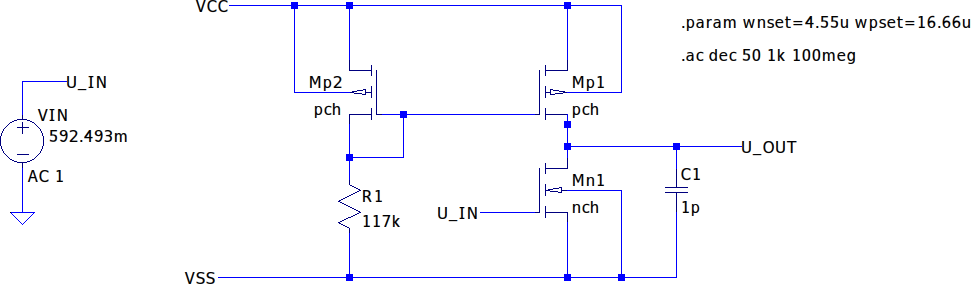
\includegraphics[scale=0.5]{4-2-2.png}
      \caption{Aktivní zátěž -- zapojení pro AC analýzu.}
      \label{fig:spice0-png}
    \end{figure}
    \begin{figure}[h!]
      \centering
      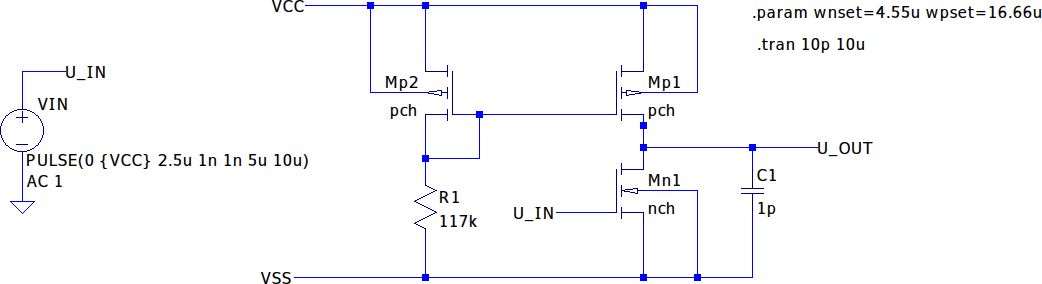
\includegraphics[scale=0.5]{4-2-3.png}
      \caption{Aktivní zátěž -- zapojení pro TRAN analýzu.}
      \label{fig:spice0-png}
    \end{figure}
\subsection{Ruční návrh}
    Rozměry trnzistoru \(M_{n1} \) ani proud obvodem se nijak nemění, nejprve na základě proudu nastavíme rozměry zbylých tranzistorů \(M_{p1,2} \):



\begin{align*}
    \frac{W_{p1,2} }{L}&=\frac{2\cdot I_{D}}{KP_{P}\cdot (U_{GS} -U_{TH})^2 } \\
    \frac{W_{p1,2} }{L}&=\frac{2\cdot \num{10e-6}}{\num{60e-6}\cdot (\num{0.2})^2 } \\
    \frac{W_{p1,2} }{L}&\doteq \num[round-mode=places,round-precision=2]{8.33} 
\end{align*}

Délku \(L=\qty{2}{\micro m}\) ponecháme a tedy \(W_{p1,2}=\qty{16.66}{\micro m} \). 

Odpor rezistoru \(R_{1} \) vypočteme z Ohmova zákona:
\begin{align*}
    R_{1} &= \frac{U_{CC} - U_{GSp2}}{I_{D} } \\
    R_{1} &= \frac{\num{1.8} - \num{0.63}}{\num{10e-6} } \\
    R_{1} &= \qty{117}{k\ohm} 
\end{align*}


\subsubsection{Simulace}
    % --- Operating Point ---

    % V(vcc):	 1.8	 voltage
    % V(u_out):	 0.900001	 voltage
    % V(u_in):	 0.592493	 voltage
    % V(n002):	 1.18964	 voltage
    % V(n001):	 0.9	 voltage
    % Id(Mn1):	 1.03976e-05	 device_current
    % Ig(Mn1):	 0	 device_current
    % Ib(Mn1):	 -9.10001e-13	 device_current
    % Is(Mn1):	 -1.03976e-05	 device_current
    % Id(Mp1):	 1.03976e-05	 device_current
    % Ig(Mp1):	 -0	 device_current
    % Ib(Mp1):	 9.09999e-13	 device_current
    % Is(Mp1):	 -1.03976e-05	 device_current
    % Id(Mp2):	 1.01679e-05	 device_current
    % Ig(Mp2):	 -0	 device_current
    % Ib(Mp2):	 6.2036e-13	 device_current
    % Is(Mp2):	 -1.01679e-05	 device_current
    % I(C1):	 9.00001e-25	 device_current
    % I(R1):	 1.01679e-05	 device_current
    % I(E1):	 0	 device_current
    % I(Vcc):	 -2.05655e-05	 device_current
    % I(Vcc2):	 0	 device_current

    \begin{figure}[h!]
        \centering
        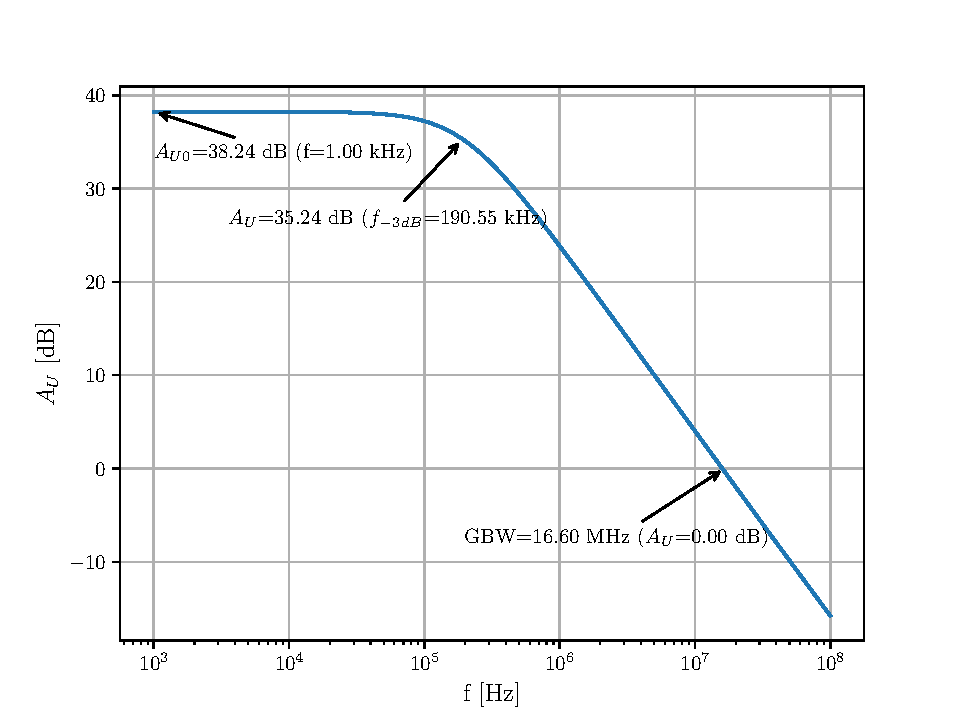
\includegraphics[width=0.8\textwidth]{4-2-2.pdf}
        \caption{AC analýza pro zesilovač s aktivní zátěží.}
        \label{fig:2-2-pdf}
    \end{figure}

    Kontrolní výpočet GBW ze simulovaných hodnot:
\begin{align*}
    GBW &= A_{U0}\cdot f_{-3dB} \\
    GBW &= 10^{\frac{\num{38.24}}{20}}\cdot \num{190.55e3} \\
    GBW &= \qty{15.560}{MHz} \\
\end{align*}

\begin{figure}[h!]
    \centering
    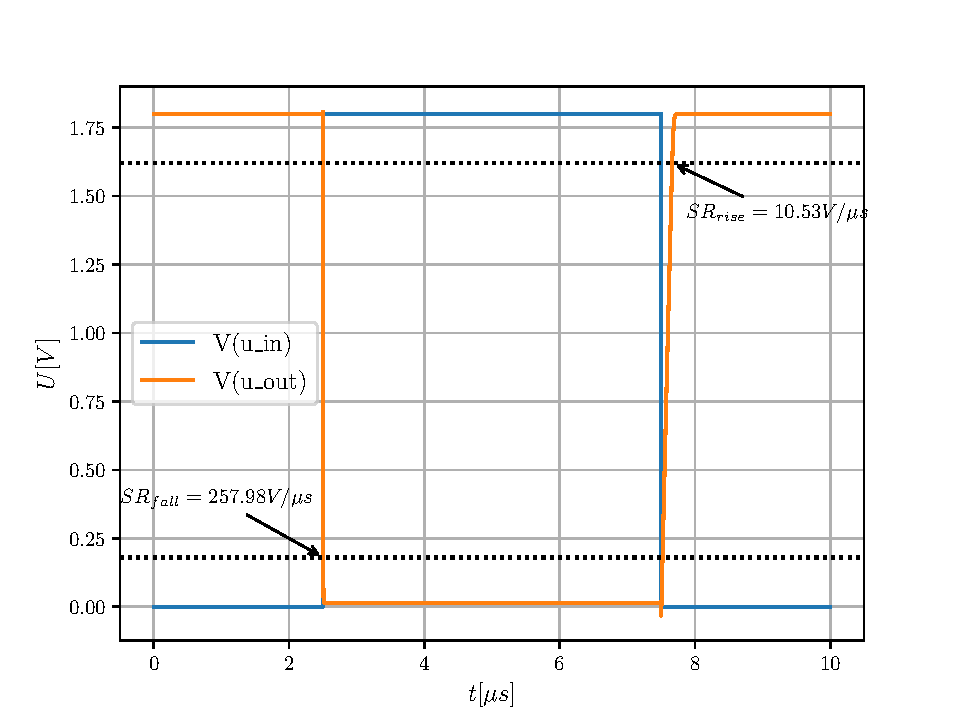
\includegraphics[width=0.8\textwidth]{4-2-3.pdf}
    \caption{TRAN analýza pro zesilovač s aktivní zátěží.}
    \label{fig:2-2-pdf}
\end{figure}



